\documentclass[varwidth=true, border=2pt]{standalone}
\usepackage{tikz}
\usetikzlibrary{calc}
\usepackage{amsmath,amssymb}

\begin{document}
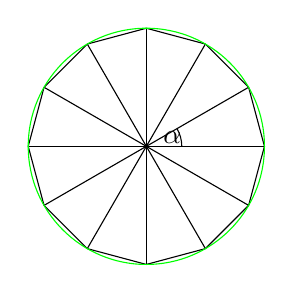
\begin{tikzpicture}
    \newcommand{\R}{1.5} % radius of the circle
    \newcommand{\n}{12} % edges of the polygon

    % Center
    \path ( 0,0) coordinate (M);

    % Inner polygon
    \foreach \nr in {1, ..., \n}{
        \path (360/\n*\nr:\R) coordinate (i\nr);
        \draw (M) -- (i\nr);
    }
    \draw (0:0.3*\R) arc (0:360/\n:0.3*\R);
    \coordinate[label=right:$\alpha$] (Alpha) at ({2*360/(\n+2)}:0.1*\R);
    \draw (i1) \foreach \i in {2,...,\n} {-- (i\i)} -- cycle;

    % Circle
    \draw[green] (0,0) circle (\R);

\end{tikzpicture}
\end{document}
